% Pursuing Stacks (cotes 134-2 to 134-8): archive cote 134-3, site page 44 (PDF page 45), typescript page 44.
% typescript. Draft compared: ps2.tex:2178-2237.
% AI-transcribed by Claude Opus 5.5 (claude-opus-5-5, adaptive thinking, effort high), Message Batches API, batch ps1 (msgbatch_01Rv5hCaNTtUt4JHx1yqoHPL), 2026-11-12; image review recorded in records/CHECK_DECISIONS_134_3_4.tsv.
\scanpage{134-3/44}
\mspage{44}
\xout{For any topos.}
There is a strong temptation now to diverge from test categories,\hand{\textbackslash}to
\margin{\unsure{--}}expanding on intrinsic versions of conditions  T 1) to T 3) for any topos,
and extract a notion of a (strictly) modelizing topos,  generalizing the
``elementary \xout{\unsure{topos}}\inserted[typed]{modelizers''} $A^{\hand{\wedge}}$ defined by strict test categories A.  But it seems
more to the point for the time being looking more closely to the one condi-%
tion,  namely T 2),  which does not appear so far as necessary for A being
a test category  -  and I suspect it is \uline{not} necessary indeed,  as no idea
occured to me how to deduce it\hand{(}\inserted{34}\xout{\illegible{1}}\hand{)}. ( I have no idea of how to make a coun-%
terexample though,  as I don't see any other way to check a category A is
a test category,  except precisely using \xout{the}\inserted[typed]{yesterday's} criterion via T 1\hand{)}to T 3\hand{)}.\hand{)}
Still I want to emphasize about the fact that T 2) \uline{is indeed a very natural}
\uline{condition}.  In this connection,  it is timely to remember that in the cate-%
\margin{\diagram{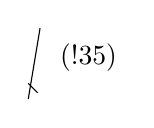
\begin{tikzpicture}[baseline=(n.base)]\draw (0,-.35)--(.15,.55);\draw (0,-.15)--(.12,-.27);\node[anchor=west] (n) at (.28,.18) {(!35)};\end{tikzpicture}}}gory (Hot),  finite direct and inverse limits exist\deleted{\illegible{1}}(and even infinite one
I guess,  but I feel I'll have to be a little careful about these ...).
T\hand{h}e existence of such limits,  in terms of the description of (Hot) as a
category of fractions of (Cat),  does'nt seem at all a trivial fact,  for
the time being I'll admit it as \xout{a} ``well known'' (\xout{in}\inserted[typed]{from} the semisimplicial set-%
up,  say),  and probably come back upon this with some care later.  Now if
\xout{a} (M,W) is any modelizer,  hence endowed with a localization functor
\[ M \hand{$\longrightarrow$} (\mathrm{Hot}) \ , \]
it is surely not irrelevant to ask about which limits this functor commu-%
tes with,  and study the case with care.  Thus in no \inserted[typed]{practical} example I know of
does this functor commute with binary amalgamated sums o\over{f}{r} \inserted{with} fibere\over{a}{d} products,
without an extra condition on at least one of the two arrows involved in
M  -  a condition of the type that one of these is a mo\over{i}{n}omorphism or a
c\over{\unsure{o}}{o}fibration (for co-products),  or a fibration (for products).  However,
in all cases known,  it seems that the functor commutes to (finite,  say)
sums and products.  For sums,  it really seems hard to make a sense out of
a localizing functor  M\hand{$\longrightarrow$}(Hot),  namely playing a ``model'' game,  without
the functor commuting at the very least to these !  In this respect,  it
is reassuring to notice that for any category A ,  the associated functors
$i_A$, $j_A$ between  $A^{\hand{\wedge}}$ and (Cat) do indeed both commute with (arbitrary) sums
-  which of course is trivial anyhow for $i_A$ (commuting to arbitrary direct
limits),  and easily checked for $j_A$ (who apparently does not commute to any
other type of direct limits,  but of course commutes with arbitrary inverse
limits).  Now for products too,  it is current use to look at products of
``models'' for homotopy types,  as models for the product type  -  so much so
that this fact is surely tacitly used everywhere\hand{,} without any feeling of
a need to comment.  It seems too that any categories M which one has looked
at so far for possible use as a category of ``models'' in one sense or other
